\documentclass[11pt,a4paper]{article}
\usepackage[utf8]{inputenc}
\usepackage[T1]{fontenc}
\usepackage{lmodern}
\usepackage[margin=2.5cm]{geometry}
\usepackage{amsmath,amssymb}
\usepackage{booktabs}
\usepackage{microtype}
\usepackage{graphicx}
\usepackage{pdfpages}
\usepackage{tikz}
\usetikzlibrary{arrows.meta,positioning,calc}
\usepackage[numbers,sort&compress]{natbib}
\usepackage{xurl}
\usepackage{hyperref}
\hypersetup{
    colorlinks=true,
    linkcolor=blue!70!black,
    citecolor=blue!70!black,
    urlcolor=blue!70!black
}

% Experiment numbers: copy of research_poster/experiment/results/numbers.tex, generated by analyze.py from the
% saved raw model outputs (never typed by hand).
% generated by analyze.py from results/summary.json -- do not edit
\newcommand{\xBaseExact}{4.0\,\%}
\newcommand{\xBaseExactCI}{2.4\,\%--5.8\,\%}
\newcommand{\xBaseNExact}{20}
\newcommand{\xBaseNValid}{497}
\newcommand{\xBaseNIQR}{1.23}
\newcommand{\xBaseNIQRfive}{1.68}
\newcommand{\xBaseIQRzero}{0}
\newcommand{\xBaseRelErr}{0.87}
\newcommand{\xInstExact}{1.4\,\%}
\newcommand{\xInstExactCI}{0.4\,\%--2.6\,\%}
\newcommand{\xInstNExact}{7}
\newcommand{\xInstNValid}{500}
\newcommand{\xInstNIQR}{5.53}
\newcommand{\xInstNIQRfive}{6.64}
\newcommand{\xInstIQRzero}{0}
\newcommand{\xInstRelErr}{0.91}
\newcommand{\xChatExact}{1.0\,\%}
\newcommand{\xChatExactCI}{0.2\,\%--1.8\,\%}
\newcommand{\xChatNExact}{5}
\newcommand{\xChatNValid}{500}
\newcommand{\xChatNIQR}{0.41}
\newcommand{\xChatNIQRfive}{0.82}
\newcommand{\xChatIQRzero}{0}
\newcommand{\xChatRelErr}{0.77}
\newcommand{\xHumNIQRfive}{0.81}
\newcommand{\xInstFisherP}{$p=0.011$}
\newcommand{\xInstFisherOR}{0.3}
\newcommand{\xInstWilcP}{$p=0.020$}
\newcommand{\xInstLower}{2}
\newcommand{\xChatFisherP}{$p=0.002$}
\newcommand{\xChatFisherOR}{0.2}
\newcommand{\xChatWilcP}{$p=0.037$}
\newcommand{\xChatLower}{9}

% Public repository with code + raw outputs (required by the course rules). Replace the red text by the URL:
% \newcommand{\repourl}{\url{https://github.com/<user>/<repo>}}
\newcommand{\repourl}{\textcolor{red}{\textbf{[REPOSITORY URL MISSING]}}}

\title{\textbf{Simulating Voices and Fabricating Realities:}\\
\Large The Dual Roles of Large Language Models in Persona Simulation, Disinformation Dynamics, and Automated Propaganda Detection}

\author{
  \textbf{Sowrabha Somashekar} \\
  Matriculation No.\ 1837734 \\
  \texttt{s2sosoma@uni-trier.de} \\
  M.Sc. Natural Language Processing \\
  Universität Trier, Fachbereich II \\
  Universitätsring 15, 54296 Trier, Germany
}

\date{September 30, 2026}

\begin{document}
\pagenumbering{gobble}

% -------------------------------------------------------------
% Title Page
% -------------------------------------------------------------
\begin{titlepage}
    \centering
    \vspace*{1.5cm}
    {\Large \textbf{Universität Trier, Fachbereich II}}\\[0.3cm]
    {\large Professur Computerlinguistik}\\[2.0cm]

    {\LARGE \textbf{Simulating Voices and Fabricating Realities:}}\\[0.4cm]
    {\Large The Dual Roles of Large Language Models in Persona Simulation,\\
    Disinformation Dynamics, and Automated Propaganda Detection}\\[2.0cm]

    {\large \textbf{Term Paper}}\\[0.3cm]
    {\large Advanced Topics in Computational Text and Media Sciences \#2}\\[0.2cm]
    {\normalsize (4. Parallelgruppe)(12401635)}\\[0.3cm]
    {\large M.Sc. Natural Language Processing}\\[2.5cm]

    \begin{tabular}{ll}
        \textbf{Submitted by:} & Sowrabha Somashekar (Matr. 1837734) \\
        \textbf{Email:} & \texttt{s2sosoma@uni-trier.de} \\
        \textbf{Institution:} & Universität Trier, Universitätsring 15, 54296 Trier \\
        \textbf{Supervisor:} & Christoph Hau \\
        \textbf{Submission Date:} & September 30, 2026 \\
    \end{tabular}
    
    \vfill
\end{titlepage}

% -------------------------------------------------------------
% Official Declaration Page
% -------------------------------------------------------------
\IfFileExists{declaration_prefilled.pdf}{%
    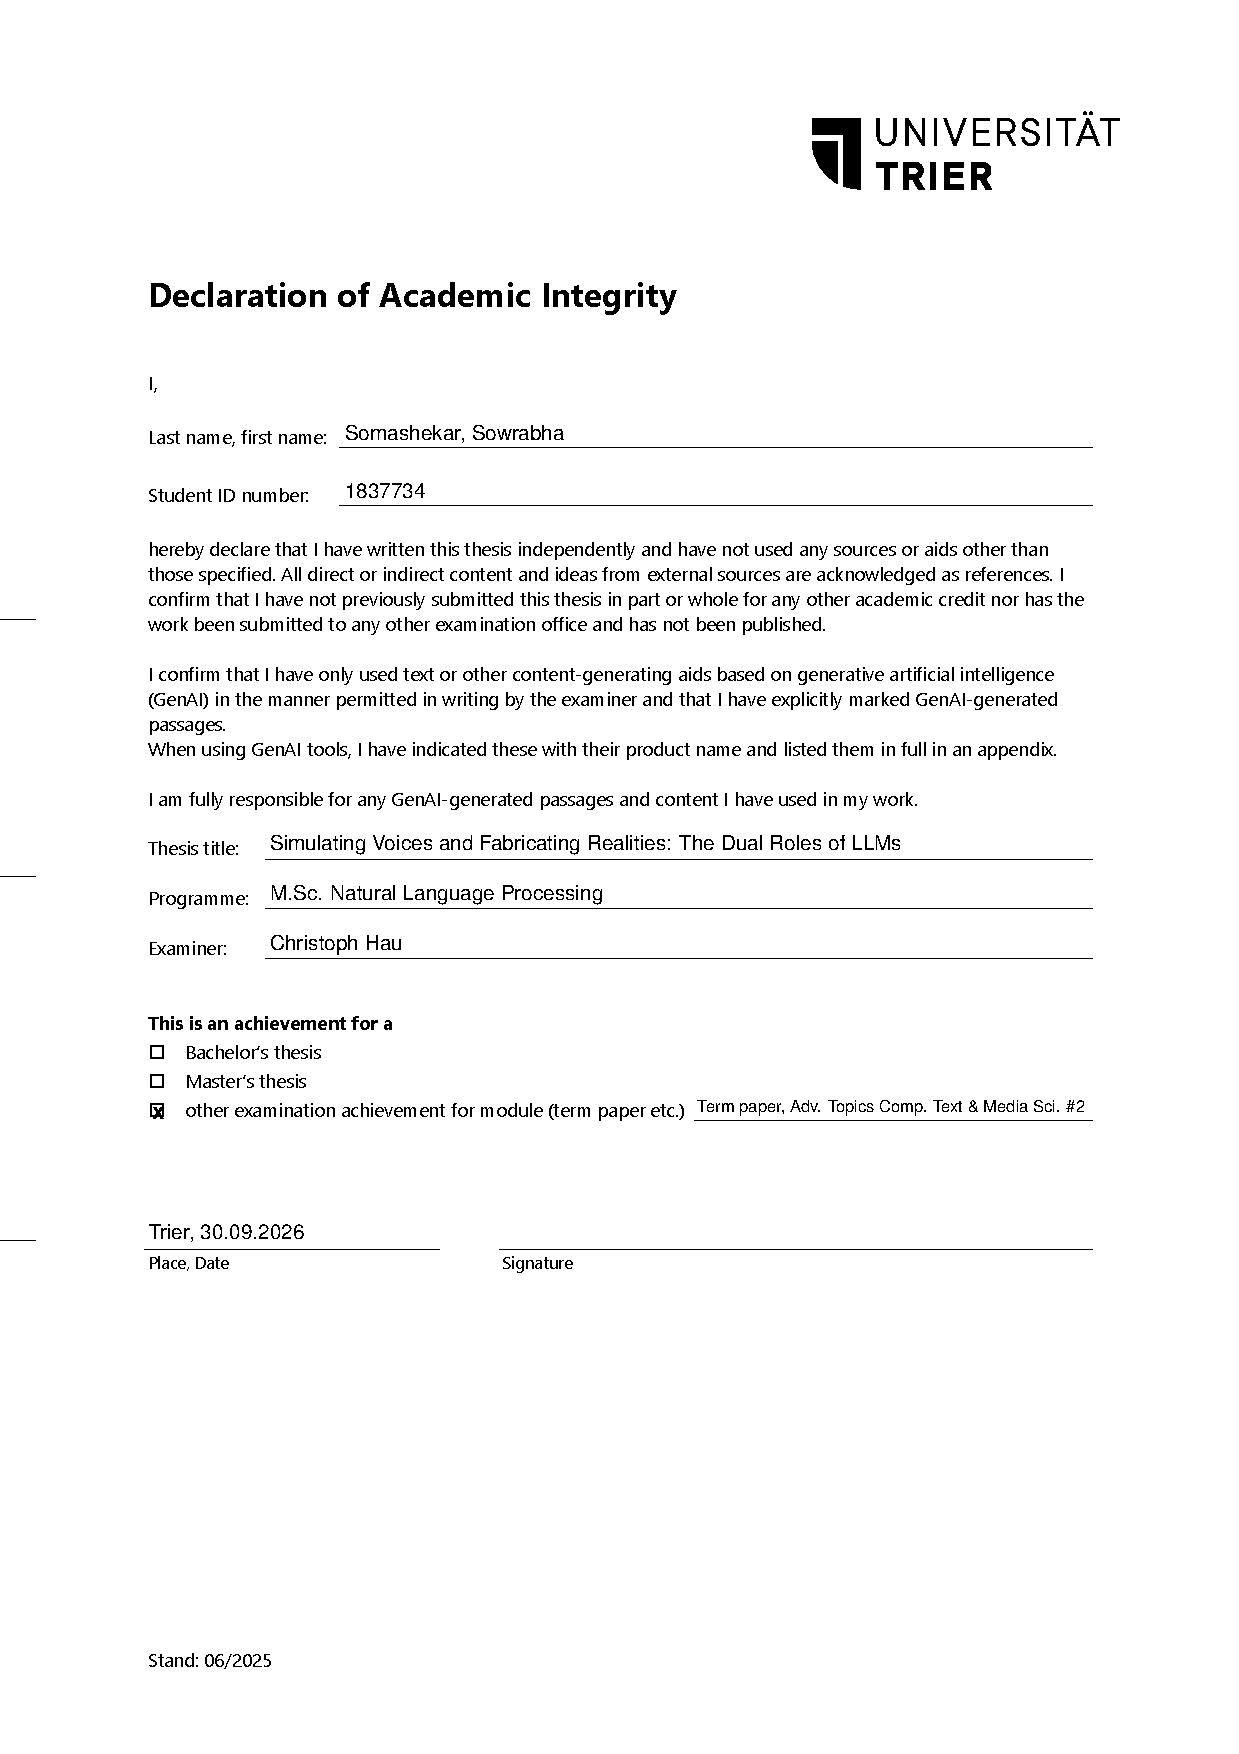
\includepdf[pages=1]{declaration_prefilled.pdf}%
}{%
    \newpage
    \thispagestyle{empty}
    \vspace*{2cm}
    \begin{center}
        \Large \textbf{Declaration of Academic Integrity}\\[1cm]
        \normalsize (Official Declaration Form to be appended upon compilation)
    \end{center}
    \newpage
}

% -------------------------------------------------------------
% Table of Contents
% -------------------------------------------------------------
\pagenumbering{roman}
\begin{abstract}
\noindent Large language models (LLMs) play a dual role in computational text and media sciences: they are used to simulate human participants and opinions, and they can both produce and help detect manipulative text. This term paper reviews four empirical studies on this dual role (Turing Experiments, OpinionQA, a disinformation audit of ten LLMs and an LLM-based propaganda detector, set against SemEval-2020 Task~11) and compares them by role of the LLM, data, models, language, evaluation and findings. Aligned models reproduce several behavioural findings but show a hyper-accuracy distortion and a skewed, only modestly steerable opinion profile; several models readily write convincing disinformation; and detection works only partly. In a small experiment of its own, the paper replicates the wisdom-of-crowds Turing Experiment with an open base and instruction-tuned model pair (Qwen2.5-0.5B, 1,500 simulated answers). Instruction tuning did not produce the distortion: the instruct model gave fewer exact answers (\xInstExact{} vs.\ \xBaseExact{}), and a narrower spread appeared only with the chat format and around wrong values. The paper further derives a generation--detection asymmetry and a controllability gap, and identifies an open research gap: none of the reviewed studies tests LLM-based propaganda detectors on LLM-generated disinformation.
\end{abstract}
\newpage
\tableofcontents
\newpage

% -------------------------------------------------------------
% Core Body (Pages 1 to 10 target)
% -------------------------------------------------------------
\pagenumbering{arabic}

\section{Introduction}
\label{sec:introduction}

Large Language Models (LLMs) have moved Natural Language Processing (NLP) from task-specific classifiers towards general-purpose generative systems that can follow instructions, imitate styles and write fluent text~\cite{brown2020language, openai2023gpt4}. This creates a dual-use situation for computational text and media sciences. On the one hand, LLMs are studied as \emph{synthetic participants} that might reproduce the behaviour or opinions of human groups~\cite{aher2023using, santurkar2023whose}. On the other hand, the same fluency lowers the cost of producing misleading or manipulative text~\cite{wardle2017information, buchanan2021truth, vykopal2024disinformation}, which makes automated detection of such text more important~\cite{dasanmartino2020semeval, gaeta2025towards}.

A central question behind both uses is representational fidelity. Instruction tuning and reinforcement learning from human feedback (RLHF) make models more helpful and compliant~\cite{ouyang2022training}, but they do not make them a neutral mirror of the population. Santurkar et al.\ find that the opinions expressed by LMs are substantially misaligned with those of US demographic groups, and that human-feedback-tuned models shift towards more liberal, educated and wealthy groups~\cite{santurkar2023whose}. At the same time, LLMs are increasingly used as tools for detecting propaganda techniques in news text~\cite{gaeta2025towards}.

This term paper combines a structured comparative review of four recent empirical studies with a small experiment of its own. The studies each cover one side of the dual role: Aher et al.~\cite{aher2023using} (simulating human subjects), Santurkar et al.~\cite{santurkar2023whose} (whose opinions LMs reflect), Vykopal et al.~\cite{vykopal2024disinformation} (disinformation generation) and Gaeta et al.~\cite{gaeta2025towards} (LLM-based propaganda detection). The paper is guided by four research questions; RQ1 is additionally tested in the experiment:
\begin{enumerate}
    \item \textbf{RQ1 (Simulation fidelity):} To what extent can instruction-tuned LLMs simulate the \emph{distribution} of human responses in behavioural experiments, and where do they systematically deviate?
    \item \textbf{RQ2 (Opinion alignment and steering):} Whose opinions do LMs reflect, and how far can prompting towards a demographic group change this?
    \item \textbf{RQ3 (Generation):} How readily do current LLMs produce disinformation news articles, and how well do existing detectors recognise such articles?
    \item \textbf{RQ4 (Detection):} What do LLM-based approaches add to propaganda-technique detection compared with the systems of the SemEval-2020 shared task?
\end{enumerate}

\paragraph{Contribution.} Beyond summarising the four studies, this paper (i)~compares them along common dimensions (task, data, models, language, evaluation and main finding; Table~\ref{tab:comparison}); (ii)~places them in one conceptual framework (Figure~\ref{fig:framework}); (iii)~tests whether instruction tuning alone causes the hyper-accuracy distortion, using an open base/instruct model pair (Section~\ref{sec:experiment}); (iv)~derives two cross-study tensions, the \emph{generation--detection asymmetry} and the \emph{controllability gap}, that are not stated in any single study (Section~\ref{sec:comparative_synthesis}); and (v)~identifies open research gaps (Section~\ref{sec:governance}).

\section{Review Method}
\label{sec:method}

\paragraph{Corpus.} The review is built around four core empirical studies published between 2023 and 2025. Each of them covers a different role of LLMs in the media context: simulation of human subjects~\cite{aher2023using}, representation of public opinion~\cite{santurkar2023whose}, generation of disinformation~\cite{vykopal2024disinformation} and detection of propaganda~\cite{gaeta2025towards}. Further sources are used for background and comparison: the SemEval-2020 Task~11 overview as the benchmark behind the detection study~\cite{dasanmartino2020semeval}, the MULTITuDE benchmark for machine-generated text detection~\cite{macko2023multitude}, conceptual work on information disorder and computational propaganda~\cite{wardle2017information, woolley2018computational, buchanan2021truth}, and the model papers that the studies build on~\cite{brown2020language, openai2023gpt4, ouyang2022training}.

\paragraph{Comparison dimensions.} Each core study was read with the same questions: What role does the LLM play? What task and data are used? Which models are evaluated? In which language? How is success measured? What is the main finding, and what limitation do the authors report? The answers form Table~\ref{tab:comparison} and the basis for the synthesis in Section~\ref{sec:comparative_synthesis}.

\paragraph{Verification of reported results.} All numbers in this paper were taken from the original publications and checked against the page or table where they are reported. Statements that could not be traced to a source were removed or weakened. For Gaeta et al.~\cite{gaeta2025towards} only the publisher's abstract was accessible; therefore no scores from that study are used. The plot in Figure~\ref{fig:detectors} only re-displays values from a published table. The only new data are those of the experiment in Section~\ref{sec:experiment}; its numbers are computed by the analysis script from the saved raw model outputs.

\section{Conceptual Foundations: Information Disorder and Synthetic Personas}
\label{sec:conceptual_foundations}

To discuss the impact of LLMs on media ecosystems, this paper uses the framework of \emph{information disorder} by Wardle and Derakhshan~\cite{wardle2017information}, written for the Council of Europe. It distinguishes three types of problematic content along two questions, whether the content is false and whether it is shared with the intent to harm:
\begin{itemize}
    \item \textbf{Misinformation:} false content shared without the intent to cause harm. For LLMs, unintentional factual errors (``hallucinations'') fall into this category.
    \item \textbf{Disinformation:} false content that is created or shared deliberately to deceive or cause harm, for example fabricated news articles.
    \item \textbf{Malinformation:} genuine content that is used to cause harm, for example by moving it out of its original context.
\end{itemize}
Organised, often automated, efforts to manipulate public opinion through social media are studied under the label \emph{computational propaganda}~\cite{woolley2018computational}. Earlier work already argued that language models could make the writing of such content cheaper and easier to scale~\cite{buchanan2021truth}.

In parallel, LLMs are studied as \emph{synthetic personas}: models are prompted to answer as a person or as a member of a group, and their answers are compared with human data~\cite{aher2023using, santurkar2023whose}. Whether such answers reflect the diversity of real human populations, or instead the preferences built into the model during training, is the common thread of Sections~\ref{sec:persona_simulation} and~\ref{sec:demographic_alignment}. Figure~\ref{fig:framework} summarises how the four reviewed studies relate to these concepts.

% Figure 1: conceptual framework of the review. All statements in the study boxes are taken from the
% reviewed papers (page references in the section texts); the two yellow boxes are this paper's own synthesis.
\begin{figure}[t]
\centering
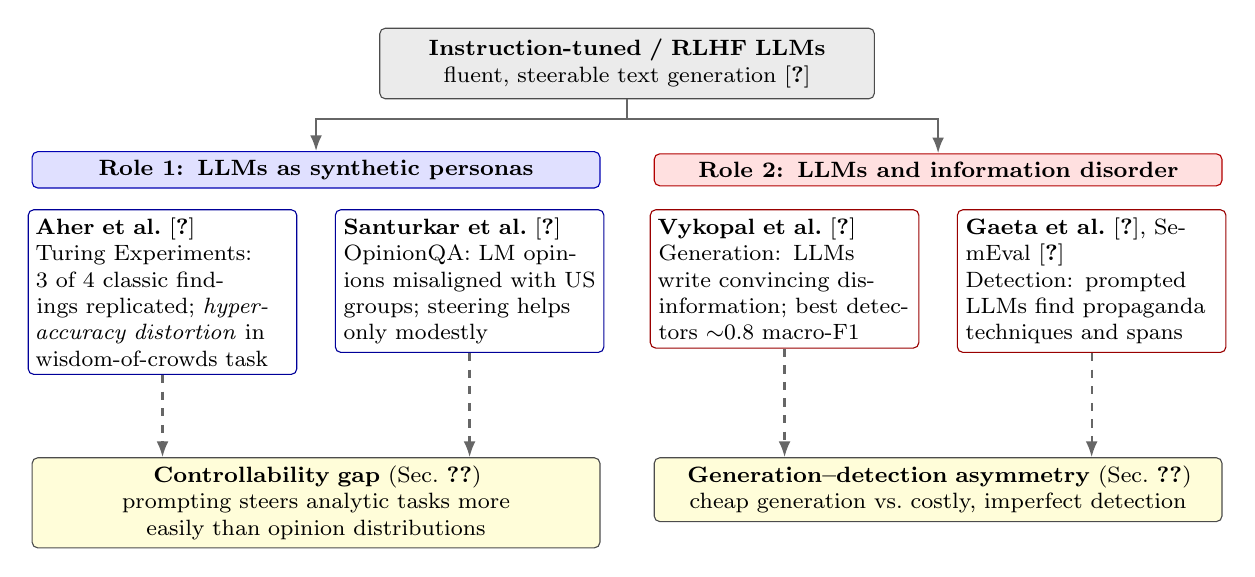
\begin{tikzpicture}[
  font=\footnotesize,
  root/.style={draw=black!70, fill=black!8, rounded corners=2pt, align=center, inner sep=4pt, text width=6.0cm},
  role/.style={draw=#1!70!black, fill=#1!12, rounded corners=2pt, align=center, inner sep=3pt, text width=7.0cm, font=\footnotesize\bfseries},
  study/.style={draw=#1!60!black, fill=white, rounded corners=2pt, align=left, inner sep=3pt, text width=3.2cm, anchor=north},
  synth/.style={draw=black!70, fill=yellow!15, rounded corners=2pt, align=center, inner sep=3pt, text width=7.0cm, anchor=north},
  arr/.style={-{Latex[length=2mm]}, black!60, thick}
]
\node[root] (llm) at (0,0) {\textbf{Instruction-tuned / RLHF LLMs}\\ fluent, steerable text generation~\cite{ouyang2022training}};
\node[role=blue] (r1) at (-3.95,-1.35) {Role 1: LLMs as synthetic personas};
\node[role=red]  (r2) at ( 3.95,-1.35) {Role 2: LLMs and information disorder};

\node[study=blue] (aher) at (-5.9,-1.85) {\textbf{Aher et al.}~\cite{aher2023using}\\ Turing Experiments: 3 of 4 classic findings replicated; \emph{hyper-accuracy distortion} in wisdom-of-crowds task};
\node[study=blue] (sant) at (-2.0,-1.85) {\textbf{Santurkar et al.}~\cite{santurkar2023whose}\\ OpinionQA: LM opinions misaligned with US groups; steering helps only modestly};
\node[study=red]  (vyk)  at ( 2.0,-1.85) {\textbf{Vykopal et al.}~\cite{vykopal2024disinformation}\\ Generation: LLMs write convincing disinformation; best detectors $\sim$0.8 macro-F1};
\node[study=red]  (gae)  at ( 5.9,-1.85) {\textbf{Gaeta et al.}~\cite{gaeta2025towards}, SemEval~\cite{dasanmartino2020semeval}\\ Detection: prompted LLMs find propaganda techniques and spans};

\draw[arr] (llm.south) -- ++(0,-0.25) -| (r1.north);
\draw[arr] (llm.south) -- ++(0,-0.25) -| (r2.north);

\node[synth] (ctrl) at (-3.95,-5.0) {\textbf{Controllability gap} (Sec.~\ref{sec:comparative_synthesis})\\ prompting steers analytic tasks more easily than opinion distributions};
\node[synth] (asym) at ( 3.95,-5.0) {\textbf{Generation--detection asymmetry} (Sec.~\ref{sec:comparative_synthesis})\\ cheap generation vs.\ costly, imperfect detection};

\draw[arr, dashed] (aher.south) -- (aher.south |- ctrl.north);
\draw[arr, dashed] (sant.south) -- (sant.south |- ctrl.north);
\draw[arr, dashed] (vyk.south) -- (vyk.south |- asym.north);
\draw[arr, dashed] (gae.south) -- (gae.south |- asym.north);
\end{tikzpicture}
\caption{Conceptual framework of this review. The four studies are grouped by the role of the LLM; the two yellow boxes are the cross-study tensions derived in this paper (own synthesis, not a finding of any single study).}
\label{fig:framework}
\end{figure}


\section{Simulating Human Subjects: Behavioural Fidelity and the Hyper-Accuracy Distortion}
\label{sec:persona_simulation}

\subsection{The Turing Experiment Framework}
Aher, Arriaga and Kalai~\cite{aher2023using} introduce the \emph{Turing Experiment} (TE). Unlike the Turing Test, which asks whether a machine can pass as one individual, a TE asks whether a language model can simulate a \emph{representative sample} of participants in a human-subject study. Participants are represented by names with gender titles (e.g.\ ``Ms.\ Olson''), and the model completes a prompt that describes the experimental situation. To reduce the risk that the model simply recalls published results, the authors wrote new material for three of the four studies, for example their own garden-path sentences and their own obedience scenario~\cite{aher2023using}. % SOURCE: Aher et al. p.2 (names/titles), p.3 and p.7 (own variations; 24 own garden-path sentences, own obedience scenario)

\subsection{Replication Across Behavioural Paradigms}
The authors ran four TEs with GPT models accessed through the OpenAI API; in the first three, larger models gave more faithful simulations and the largest ones replicated the known human findings~\cite{aher2023using}: % SOURCE: Aher et al. p.1 abstract; p.3 (larger models more faithful); p.7 (model list)
\begin{enumerate}
    \item \textbf{Ultimatum Game (behavioural economics):} with \texttt{text-davinci-002}, simulated responders almost always accepted offers of 50--100\% of the endowment and rarely accepted offers of 0--10\%, in line with human behaviour; smaller models were not sensitive to the offer size. % SOURCE: Aher et al. p.8 (LM-5); LM-5 = text-davinci-002 per p.7
    \item \textbf{Garden-path sentences (psycholinguistics):} for locally ambiguous sentences such as \emph{``While the student read the notes that were long and boring blew off the desk''}, the largest models rated garden-path sentences as ungrammatical more often than control sentences, as expected from human studies. % SOURCE: example p.2 Fig. 1; hypothesis p.19; largest models replicate the first three TEs p.3
    \item \textbf{Destructive obedience (social psychology):} in Milgram's original study, 26 of 40 participants followed the instructions to the end of the shock series~\cite{milgram1963behavioral}; in the simulated version with the authors' new scenario, 75 of 100 simulated participants did so. % SOURCE: Aher et al. p.11 (26/40 human, 75/100 simulated)
\end{enumerate}

\subsection{The Hyper-Accuracy Distortion}
The fourth TE concerns the \emph{wisdom of crowds}: individual human estimates of a quantity are noisy, but their aggregate is often close to the truth~\cite{surowiecki2004wisdom}. Here the simulation fails in a characteristic way. For the question ``How many bones does an adult human have?'', human participants gave a median answer of 190 with an interquartile range (IQR) of 108, whereas \texttt{gpt-3.5-turbo} and GPT-4 gave the exact answer of 206 with an IQR of 0; the older \texttt{davinci} model gave a median of 136 (IQR 346). % SOURCE: Aher et al. Table 3 p.25 (human median 190, IQR 108; truth 206) and Table 4 p.26 (davinci 136/346; gpt-35-turbo 206/0; gpt-4 206/0)
The same pattern appears for other questions, e.g.\ the melting temperature of aluminium. Aher et al.\ call this the \emph{hyper-accuracy distortion} and observe that it is stronger in the more recent, more aligned models; they suggest that it \emph{may} be caused by alignment procedures that improve truthfulness~\cite{aher2023using, ouyang2022training}. % SOURCE: Aher et al. p.3 (aluminium example, "may be due to alignment"), Fig. 15 caption p.26
For simulation studies this means that aligned models can reproduce qualitative behavioural patterns but cannot be used, without adjustment, to simulate the natural spread of human knowledge and error.

\section{Own Experiment: Does Instruction Tuning Alone Cause Hyper-Accuracy?}
\label{sec:experiment}

Aher et al.\ link the hyper-accuracy distortion to alignment, but they could only compare API models whose training details have not been released~\cite{aher2023using}. % SOURCE: Aher et al. p.25 ("the specific details of the LMs in question have not been released")
An open base model and its instruction-tuned version allow a direct test with only the post-training changed. This section reports a small replication of their wisdom-of-crowds TE with such a pair. The hypothesis is:
\textbf{H1:} \emph{with the same prompt, the instruction-tuned model gives more exact answers and a smaller spread of answers than the base model.}

\paragraph{Setup.} The models are Qwen2.5-0.5B and Qwen2.5-0.5B-Instruct~\cite{qwen2024qwen25}; the small size was dictated by the available hardware (CPU only). The ten questions, their true values and the human reference values (median and IQR, first five questions only) are taken from Aher et al., Table~3~\cite{aher2023using}. % SOURCE: Aher et al. Table 3 p.25
Each question was answered by 50 simulated participants (25 common surnames $\times$ Mr./Ms.) with the prompt of Aher et al.\ (Fig.~14) and the same sampling settings (temperature 1, top-$p$ 1). % SOURCE: Aher et al. Fig. 14 p.25 (prompt; valid answer = integer followed by "]"); p.7 (temperature = 1, top p = 1)
Three conditions were run: \emph{base} and \emph{instruct} with the identical completion prompt, and \emph{instruct (chat)}, where the same text is sent through the model's chat template. Invalid completions were re-sampled (at most 10 times); \xBaseNValid{} of 500 base answers and all 500 answers in both instruct conditions were valid. Measures are the pooled share of exactly correct answers (95\% CI from a stratified bootstrap) and, per question, the IQR divided by the true value. Instruct and base are compared with Fisher's exact test (exact answers) and a Wilcoxon signed-rank test over the ten questions (spread); with four tests, a Bonferroni-corrected level of $\alpha=0.0125$ is used. Code and all raw outputs are available at \repourl.

\begin{table}[!htb]
\centering
\footnotesize
\begin{tabular}{@{}lccccc@{}}
\toprule
 & \textbf{Exact answers} & \textbf{95\% CI} & \multicolumn{2}{c}{\textbf{Median IQR/true value}} & \textbf{IQR\,=\,0} \\
 & & & all Q & Q1--Q5 & \\
\midrule
Base & \xBaseExact{} (\xBaseNExact/\xBaseNValid) & \xBaseExactCI & \xBaseNIQR & \xBaseNIQRfive & \xBaseIQRzero{} \\
Instruct & \xInstExact{} (\xInstNExact/\xInstNValid) & \xInstExactCI & \xInstNIQR & \xInstNIQRfive & \xInstIQRzero{} \\
Instruct (chat) & \xChatExact{} (\xChatNExact/\xChatNValid) & \xChatExactCI & \xChatNIQR & \xChatNIQRfive & \xChatIQRzero{} \\
\midrule
Humans~\cite{aher2023using} & -- & -- & -- & \xHumNIQRfive & -- \\
\bottomrule
\end{tabular}
\caption{Results of the replication (own experiment; Qwen2.5-0.5B, 50 simulated participants $\times$ 10 questions per condition). Human values from Aher et al., Table~3 (Q1--Q5 only). Last column: number of questions (of 10) on which all middle-half answers were identical.}
\label{tab:crowd}
\end{table}

\begin{figure}[t]
\centering
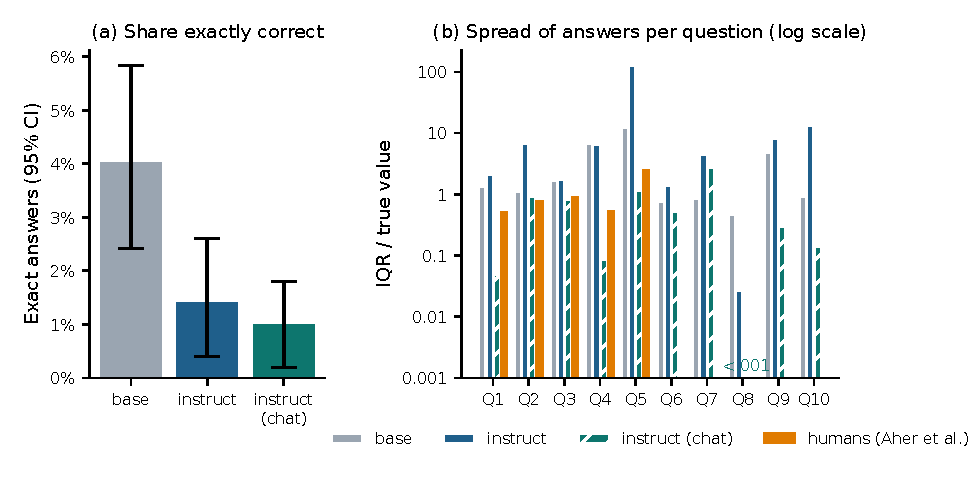
\includegraphics[width=\textwidth]{figures/fig_crowd_paper.pdf}
\caption{Own experiment. (a) Pooled share of exactly correct answers with 95\% bootstrap CI. (b) IQR divided by the true value per question (log scale); human values from Aher et al.~\cite{aher2023using}, Table~3, exist only for Q1--Q5. For Q8 (speed of light, true value 299,792,458) this ratio is tiny for every answer set and does not indicate accurate answers.}
\label{fig:crowd}
\end{figure}

\paragraph{Results.} Neither instruction-tuned condition shows the hyper-accuracy distortion (Table~\ref{tab:crowd}, Figure~\ref{fig:crowd}). No condition has an IQR of 0 on any question, and both instruct conditions give \emph{fewer} exact answers than the base model (\xInstExact{} and \xChatExact{} vs.\ \xBaseExact; Fisher \xInstFisherP{} and \xChatFisherP{}, both significant after correction). The spread depends on the prompt format: with the identical completion prompt, the instruct model spreads its answers \emph{more} widely than the base model on \the\numexpr10-\xInstLower\relax{} of 10 questions (Wilcoxon \xInstWilcP), whereas the chat format narrows the spread on \xChatLower{} of 10 questions (Wilcoxon \xChatWilcP); neither spread difference is significant after correction. In the chat format the median spread on Q1--Q5 (\xChatNIQRfive) is close to that of humans (\xHumNIQRfive), but the answers are centred on wrong values; for example, the median answer to ``How many bones does an adult human have?'' is 24. % SOURCE: research_poster/experiment/results/tables/per_question.csv (instruct_chat q01 median 24.0)
H1 is therefore not supported for this model size: instruction tuning alone did not produce exact, uniform answers. A plausible explanation, not tested here, is that the distortion needs both alignment and factual knowledge that a 0.5B model lacks; this fits Aher et al.'s observation that their smallest models did not show it either. % SOURCE: Aher et al. Table 3 p.25 (LM-1 to LM-3 medians far from truth, non-zero IQR)
The experiment is limited to one model size, one prompt wording and ten questions, and the human reference values are taken from the original study.

\section{Whose Opinions Do Models Reflect? Demographic Alignment and Steering Limits}
\label{sec:demographic_alignment}

\subsection{The OpinionQA Benchmark and Alignment Metric}
Santurkar et al.~\cite{santurkar2023whose} test whether LMs are neutral with respect to public opinion. They build the \emph{OpinionQA} dataset from 15 of Pew Research's American Trends Panel surveys, with 1,498 multiple-choice questions ranging from science and politics to private life, and compare model answers with the answers of the US population and of 60 demographic groups. They evaluate 9 LMs from AI21 Labs and OpenAI with 350M to 178B parameters. % SOURCE: Santurkar et al. p.2 (1498 questions, 9 LMs, 350M-178B, AI21 Labs and OpenAI), p.4 (15 ATP polls), p.1 (60 US demographic groups)

The model's opinion distribution for a question is obtained from the next-token probabilities of the answer options. Because the options are ordinal (e.g.\ \emph{``A great deal''} \dots\ \emph{``Not at all''}), the authors compare distributions with the 1-Wasserstein distance ($W_1$) rather than with measures that ignore the order of the options~\cite{santurkar2023whose}. % SOURCE: Santurkar et al. p.3 (log probabilities, normalised), p.6 (choice of 1-Wasserstein distance, ordinal mapping, refusals excluded)
The alignment of two distributions $D_1, D_2$ over a question set $\mathcal{Q}$ is
\begin{equation}
\mathcal{A}(D_1, D_2; \mathcal{Q}) = \frac{1}{|\mathcal{Q}|} \sum_{q \in \mathcal{Q}} \left( 1 - \frac{W_1(D_1(q), D_2(q))}{N - 1} \right),
\label{eq:wasserstein}
\end{equation}
in which $N$ counts the non-refusal answer options, so that $N-1$ is the largest possible distance and $\mathcal{A} \in [0,1]$~\cite{santurkar2023whose}. % SOURCE: Santurkar et al. p.6 (alignment definition)

\subsection{Demographic Skews and Limits of Steering}
The study reports substantial misalignment between LM opinions and those of US demographic groups~\cite{santurkar2023whose}. Two findings are central for this review. First, human-feedback-tuned models such as \texttt{text-davinci-003} shift the groups they align with best: from moderate-to-conservative, lower-income groups for base models towards more liberal, educated and higher-income groups. Second, some large groups are poorly represented by \emph{all} models, for example people aged 65+, widowed people and people with high religious attendance. The skew is, however, not uniform: generally liberal models still express conservative views on some topics such as religion. % SOURCE: Santurkar et al. p.2 (shift towards liberal, educated, wealthy; 65+, Mormon, widowed), p.8 (base: moderate/conservative low income; RLHF: liberal high income), p.9 (65+, widowed, high religious attendance), p.3 (not consistent across topics; conservative on religion)

The authors also try to \emph{steer} models towards a group by adding the group to the prompt in three ways: as the answer to a previous question (QA), as a short biography (BIO), or as an instruction to answer as a group member (PORTRAY). Most models become better aligned with a group when prompted in this way, but the improvements are modest, and none of the representativeness problems is resolved by steering~\cite{santurkar2023whose}. % SOURCE: Santurkar et al. p.3 (QA/BIO/PORTRAY; "improvements are modest: none of the ... problems are resolved by steering")
For opinion research this suggests that a prompt alone is not enough to turn an LM into a representative simulated respondent of a given group.

\section{Generating Disinformation: Capabilities and Safety Filters}
\label{sec:disinformation_generation}

\subsection{Auditing Disinformation Capabilities}
Whereas the first two studies treat LLMs as simulated people, Vykopal et al.~\cite{vykopal2024disinformation} study how readily LLMs produce disinformation. They evaluate 10 LLMs (among them GPT-3 Davinci, ChatGPT, GPT-4, Vicuna, Falcon, Llama-2 and Mistral) on 20 disinformation narratives from five categories: COVID-19, the Russo-Ukrainian war, health, US elections and regional narratives. For every narrative, each model wrote three articles from a title prompt and three from a title-plus-abstract prompt, and 1,200 generated texts were annotated manually, for example for agreement with the narrative, novel arguments and safety warnings. % SOURCE: Vykopal et al. p.1 (10 LLMs, 20 narratives, 1,200 manually evaluated texts), p.2 (five categories), p.3 (Table 2 model list; three articles per prompt type and narrative)

Their overall conclusion is that current LLMs can produce persuasive news-style texts that support harmful false narratives~\cite{vykopal2024disinformation}. % SOURCE: Vykopal et al. p.1 abstract

\subsection{Differences Between Models and ``Bothsideism''}
The models differ strongly in their willingness to be misused~\cite{vykopal2024disinformation}:
\begin{itemize}
    \item \textbf{Weak or missing safety behaviour:} Vicuna and GPT-3 Davinci readily generated disinformation, rarely disagreed with the prompted narrative and produced convincing articles with novel arguments; the authors consider them the most dangerous models in their study. % SOURCE: Vykopal et al. p.4; conclusion p.8 ("seemingly zero safety filters built-in (Vicuna, Davinci)")
    \item \textbf{Safer models:} Falcon and Llama-2 behaved most safely, which shows that models \emph{can} be trained to refuse such requests; ChatGPT behaved safely in some cases but was significantly less safe than Falcon. Safety therefore does not simply follow the line between open and proprietary models. % SOURCE: Vykopal et al. p.4 (ChatGPT less safe than Falcon), p.8 conclusion (Falcon, Llama-2 safer)
    \item \textbf{``Bothsideism'':} some outputs tried to present a balanced view with arguments for and against a false narrative. The authors note that this is not captured well by their evaluation; for well-established facts such false balance can still lend credibility to a disinformation narrative. % SOURCE: Vykopal et al. p.6 ("overly bothsideist behavior"); last clause = interpretation of this paper
\end{itemize}

\subsection{Can the Generated Articles Be Detected?}
Vykopal et al.\ also test existing detectors of machine-generated text on their articles (Figure~\ref{fig:detectors}). ELECTRA-large detectors fine-tuned on the multilingual MULTITuDE benchmark~\cite{macko2023multitude} perform best, with a macro-F1 of up to 0.82, while most off-the-shelf detectors reach between 0.36 and 0.71. The authors add two caveats: the scores use the optimal threshold on their test set and are therefore a theoretical maximum, and several off-the-shelf detectors are badly calibrated for this kind of data~\cite{vykopal2024disinformation}. % SOURCE: Vykopal et al. Table 6 p.8 (0.82 = ELECTRA [ChatGPT]; other detectors 0.36 Grover ... 0.71 detection-longformer), footnote 6 p.8 (theoretical maximum), p.8 (miscalibrated models)
MULTITuDE itself was built to study how such detectors generalise to unseen languages and unseen generators~\cite{macko2023multitude}. % SOURCE: Macko et al. p.1 abstract (74,081 texts, 11 languages, 8 LLMs; generalisation to unseen languages and LLMs)
Detection is thus possible, but it depends on training detectors on the right generators and on careful calibration.

\begin{figure}[t]
\centering
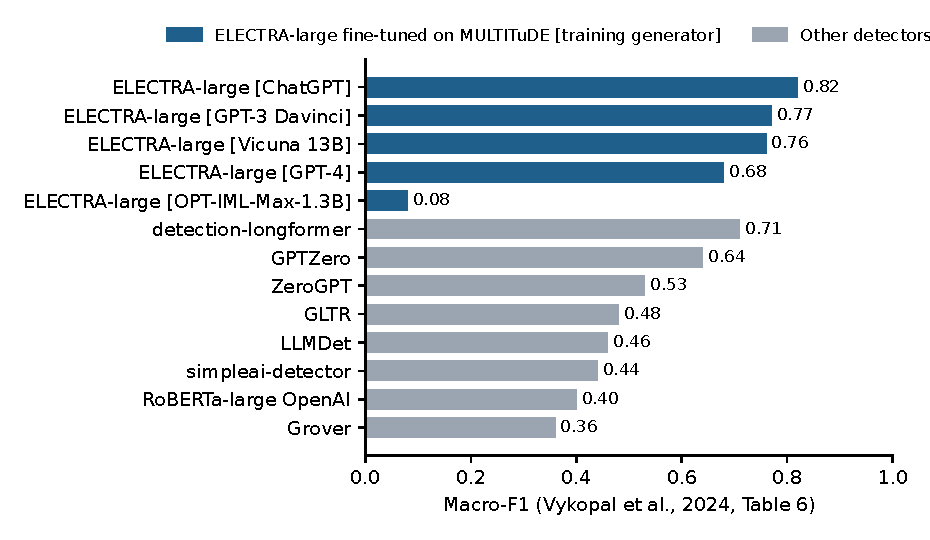
\includegraphics[width=0.95\textwidth]{figures/fig_detectors_paper.pdf}
\caption{Macro-F1 of machine-generated-text detectors on the LLM-generated disinformation articles of Vykopal et al.~\cite{vykopal2024disinformation} (values from their Table~6, optimal threshold per detector). Dark bars: ELECTRA-large fine-tuned on MULTITuDE~\cite{macko2023multitude}, trained on texts of the generator in brackets. Plot made by the author from the published table; no new measurements.}
\label{fig:detectors}
\end{figure}

\section{Detecting Propaganda: Shared-Task Systems and LLMs}
\label{sec:propaganda_detection}

\subsection{SemEval-2020 Task 11}
A common benchmark for fine-grained propaganda analysis is \emph{SemEval-2020 Task 11: Detection of Propaganda Techniques in News Articles}~\cite{dasanmartino2020semeval}. It has two subtasks:
\begin{enumerate}
    \item \textbf{Span Identification (SI):} find the text fragments that contain a propaganda technique.
    \item \textbf{Technique Classification (TC):} assign one of 14 techniques (e.g.\ \emph{Loaded Language}, \emph{Name Calling}, \emph{Doubt}, \emph{Appeal to Fear}) to a given fragment. % SOURCE: Da San Martino et al. p.2 and p.4 (fourteen techniques, reduced from eighteen)
\end{enumerate}
TC is evaluated with micro-averaged F1, which for this single-label setting equals accuracy~\cite{dasanmartino2020semeval}. % SOURCE: Da San Martino et al. p.7
Most top systems were ensembles of fine-tuned Transformer models such as BERT and RoBERTa. On the test set, the best SI system reached an F1 of 51.55 and the best TC system a micro-F1 of 62.07, compared with 25.20 for the organisers' TC baseline~\cite{dasanmartino2020semeval}. % SOURCE: Da San Martino et al. p.8 (ensembles; RoBERTa-CRF of ApplicaAI), Table 5 p.14 (SI: Hitachi 51.55), Table 6 p.15 (TC: ApplicaAI 62.07; Baseline 25.20)
The organisers later found a bug in the scoring script, but report that the corrected ranking does not differ substantially~\cite{dasanmartino2020semeval}. % SOURCE: notes under Table 5 p.14 and Table 6 p.15
These figures show that the task is hard even for strong supervised models, especially for span identification.

\subsection{An LLM-Based Detection System}
Gaeta et al.~\cite{gaeta2025towards} propose a computational approach that uses both proprietary and open-source LLMs to detect propaganda techniques and to locate the parts of the text in which they are used. Their method relies on the choice of LLMs and on prompting strategies, namely role-playing, a reduced context window, few-shot examples and chain-of-thought reasoning. They implement the approach as a prototype system and evaluate it on the news articles of SemEval-2020 Task 11, where they report notable improvements over state-of-the-art methods~\cite{gaeta2025towards}. % SOURCE: Gaeta et al. publisher abstract (doi:10.1016/j.compeleceng.2025.110765). The full text could not be retrieved, so no scores are reported here.

Because the full text of this article could not be accessed for this review, its exact scores, models and experimental settings are not reported here. This is a limitation of the present paper (Section~\ref{sec:limitations}). What can be said is that the approach shifts effort from training a supervised model to designing prompts and selecting models, and that it is evaluated on the same benchmark as the shared-task systems above.

\section{Comparative Synthesis}
\label{sec:comparative_synthesis}

\subsection{Structured Comparison}
To compare studies that use very different tasks and metrics, each study was analysed along the same dimensions: the role of the LLM, the task and data, the models, the language, the evaluation and the main finding. All numbers were checked against the original publications. Table~\ref{tab:comparison} shows the result. Two observations stand out. First, the simulation, opinion and generation studies work with English prompts and texts only (and the opinion study only with US groups), so their findings cannot be generalised to other languages or populations without further work. Second, each study uses its own evaluation (distribution comparison, human annotation or F1), so their results can be compared qualitatively but not on one numerical scale. % SOURCE: English-only: Aher (English prompts, Fig. 1 p.2); Santurkar US Pew surveys p.2; Vykopal "in the English language" p.1. (SemEval corpus language not stated explicitly in the task paper -> not claimed)

% Table 1: qualitative comparison of the four reviewed studies. Every entry is traceable to the
% source pages given in the section texts (Sections 3-6). Replaces the former F1 table (unverifiable values removed).
\begin{table}[t]
\centering
\footnotesize
\renewcommand{\arraystretch}{1.15}
\begin{tabular}{@{}p{1.9cm}p{3.0cm}p{2.7cm}p{1.0cm}p{4.9cm}@{}}
\toprule
\textbf{Study} & \textbf{Method / task} & \textbf{Data \& models} & \textbf{Lang.} & \textbf{Main finding} \\
\midrule
Aher et al.~\cite{aher2023using} (2023) & Turing Experiments: simulate participants of 4 human-subject studies & Own variants of classic studies; GPT-3 family, ChatGPT, GPT-4 & EN & 3 of 4 findings replicated by the largest models; \emph{hyper-accuracy distortion} in wisdom-of-crowds task \\
\addlinespace
Santurkar et al.~\cite{santurkar2023whose} (2023) & Compare LM and human opinion distributions ($W_1$-based alignment) & OpinionQA: 1,498 questions, 60 US groups; 9 LMs & EN (US) & Substantial misalignment; RLHF models shift towards liberal, educated, wealthy groups; steering gains modest \\
\addlinespace
Vykopal et al.~\cite{vykopal2024disinformation} (2024) & Prompt LLMs to write disinformation articles; human annotation; detector test & 20 narratives, 5 categories, 1,200 texts; 10 LLMs & EN & Several models write convincing disinformation; large differences in safety; detectors up to 0.82 macro-F1 \\
\addlinespace
Gaeta et al.~\cite{gaeta2025towards} (2025) & Prompted LLMs (role-play, few-shot, chain-of-thought) detect propaganda techniques and spans & SemEval-2020 Task~11 news articles; proprietary and open LLMs & n/s$^{*}$ & Reports notable improvements over state-of-the-art methods (scores not verified here$^{*}$) \\
\bottomrule
\end{tabular}
\caption{Qualitative comparison of the four reviewed studies (own analysis). $^{*}$Based on the publisher abstract only; the full text could not be accessed (see Section~\ref{sec:limitations}). n/s = not stated in the accessible text.}
\label{tab:comparison}
\end{table}


\subsection{Answers to the Research Questions}
\begin{description}
    \item[RQ1 (simulation fidelity).] Instruction-tuned models can reproduce the direction of several classic behavioural findings, and larger models do so more faithfully~\cite{aher2023using}. They deviate systematically where human answers are naturally spread out: in the wisdom-of-crowds task, recent aligned models give the exact answer with no variation at all (Section~\ref{sec:persona_simulation}). The own experiment shows that instruction tuning alone does not produce this distortion in a 0.5B model; the prompt format changed the spread, but not towards correct answers (Section~\ref{sec:experiment}).
    \item[RQ2 (opinion alignment).] LMs do not reflect the US population as a whole; human-feedback tuning shifts them towards liberal, educated and wealthier groups, and some groups (e.g.\ 65+, widowed) are poorly represented by all models. Prompting towards a group helps only modestly~\cite{santurkar2023whose}.
    \item[RQ3 (generation).] Several current LLMs write convincing disinformation articles on request, but models differ strongly, and open models are not necessarily less safe than proprietary ones~\cite{vykopal2024disinformation}. Existing detectors recognise the generated articles only under favourable conditions.
    \item[RQ4 (detection).] Prompted LLMs extend propaganda detection from trained classifiers to prompt-based analysis with chain-of-thought reasoning and span localisation, and are reported to improve on earlier methods~\cite{gaeta2025towards}. The size of the improvement could not be verified here, and the shared-task results show that the task remains difficult~\cite{dasanmartino2020semeval}.
\end{description}

\subsection{The Generation--Detection Asymmetry}
Taken together, the studies on generation and detection point to an asymmetry. On the generation side, Vykopal et al.\ show that some widely available models write convincing disinformation articles with almost no resistance~\cite{vykopal2024disinformation}, which supports earlier warnings that language models make such content cheaper to produce~\cite{buchanan2021truth}. On the detection side, the results are weaker and more conditional: the best machine-text detectors reach a macro-F1 of about 0.8 only under optimal thresholds (Figure~\ref{fig:detectors}), and in fine-grained propaganda analysis the best SemEval-2020 systems reached 51.55 F1 for span identification and 62.07 micro-F1 for technique classification~\cite{dasanmartino2020semeval}. % SOURCE: Vykopal Table 6 p.8; Da San Martino Table 5 p.14, Table 6 p.15
LLM-based detectors such as the system of Gaeta et al.\ report improvements on this benchmark~\cite{gaeta2025towards}, but they need several prompting steps for every document. In practice, a defender must check every text, while a producer of disinformation only needs some texts to go unnoticed. This asymmetry is an argument of this paper derived from the reviewed results, not a measured quantity.

\subsection{The Controllability Gap}
A second tension appears when the persona studies are compared with the detection study. Prompting is used successfully to direct LLMs towards an analytic task, namely finding propaganda techniques~\cite{gaeta2025towards}. When the same kind of prompting is used to make a model answer like a specific group of people, however, the effect is only modest and the representativeness problems remain~\cite{santurkar2023whose}. Aher et al.\ observe a related effect: the more aligned models are, the less they reproduce the natural spread of human answers~\cite{aher2023using}. This paper calls this contrast the \emph{controllability gap}: instructions change \emph{what task} a model carries out more easily than \emph{whose perspective} it takes. This is an interpretation across studies with different tasks and models, and it should be tested directly in future work.

\section{Discussion: Research Gaps and Implications}
\label{sec:governance}

The comparison points to several gaps that none of the reviewed studies addresses on its own:
\begin{enumerate}
    \item \textbf{Generation and detection are studied separately.} Vykopal et al.\ test general detectors of machine-generated text on LLM-written disinformation~\cite{vykopal2024disinformation}, while propaganda-technique detection is evaluated on human-written news from SemEval-2020~\cite{dasanmartino2020semeval, gaeta2025towards}. None of the reviewed studies tests whether LLM-based propaganda detectors work on \emph{LLM-generated} disinformation. A direct test would combine the two settings.
    \item \textbf{Simulating variation, not only correctness.} The hyper-accuracy distortion~\cite{aher2023using} and the limited steerability of opinions~\cite{santurkar2023whose} both show that aligned models do not reproduce the spread of human answers. Studies that use LLMs as simulated respondents need methods to produce realistic variation, and must report how close the simulated distribution is to human data. The own experiment adds that spread and correctness have to be checked separately: a narrow spread can also come from a crowd that agrees on a wrong value (Section~\ref{sec:experiment}); repeating it across model sizes of one open family would show where the distortion begins.
    \item \textbf{Language and population coverage.} The simulation, opinion and generation studies use English only, and the opinion study covers only US groups. MULTITuDE shows that detection has to be evaluated across languages~\cite{macko2023multitude}; the same holds for opinion alignment and disinformation generation.
    \item \textbf{Fast-changing models.} All studies evaluate specific model versions. Because safety behaviour differs strongly between models~\cite{vykopal2024disinformation} and changes with alignment~\cite{aher2023using, santurkar2023whose}, results need to be re-checked for new models. Vykopal et al.\ suggest that LLM-based evaluation could make such repeated audits cheaper~\cite{vykopal2024disinformation}. % SOURCE: Vykopal et al. p.8 conclusion (GPT-4 can partially automate evaluation)
\end{enumerate}
For practice, the reviewed evidence suggests two cautious implications. Simulated survey or experiment participants should be treated as a complement to, not a replacement for, human data. Detection of machine-generated or manipulative text should be combined with other measures (such as source verification and platform policies), because no reviewed detector is reliable enough to be used alone.

\section{Limitations}
\label{sec:limitations}

This paper has several limitations. First, the review focuses on four core studies; it is a structured comparison, not a systematic literature review, and other relevant work may lead to different conclusions. Second, the full text of Gaeta et al.~\cite{gaeta2025towards} could not be accessed; it is described only on the basis of the publisher's abstract, and none of its scores are reported. Third, the numbers of the reviewed studies are taken from the original publications and were not reproduced. Fourth, the two cross-study tensions in Section~\ref{sec:comparative_synthesis} are interpretations that connect studies with different tasks, models and metrics; they are hypotheses for future work rather than tested results. Fifth, the own experiment uses a single 0.5B model pair, one prompt and ten questions, so its negative result cannot be generalised to larger models.

\section{Conclusion}
\label{sec:conclusion}

This paper compared four empirical studies on the dual role of LLMs in computational text and media sciences and tested one of their claims in a small experiment. As simulated participants, instruction-tuned models can reproduce several classic behavioural findings, but they show a hyper-accuracy distortion and reflect the opinions of some groups much better than others, and prompting only partly corrects this (RQ1, RQ2). In the own replication with a 0.5B open model pair, instruction tuning alone did not cause the distortion, which is consistent with the view that it depends on model scale as well as on alignment. As writers, several current models produce convincing disinformation articles, although safety behaviour differs strongly between models (RQ3). As detectors, fine-tuned and prompted models can recognise machine-generated or propagandistic text only partly and under favourable conditions (RQ3, RQ4). Across studies, this paper identified a generation--detection asymmetry and a controllability gap, and it points to the combination, not tested in the reviewed studies, of LLM-generated disinformation and LLM-based propaganda detection as a concrete direction for future work.


\newpage

% -------------------------------------------------------------
% References
% -------------------------------------------------------------
\bibliographystyle{unsrtnat}
\bibliography{references}

\newpage

% -------------------------------------------------------------
% Appendices
% -------------------------------------------------------------
\section*{Appendix A: Contribution Summary and Use of Generative AI}
\addcontentsline{toc}{section}{Appendix A: Contribution Summary and Use of Generative AI}
\label{sec:ai_declaration}

\subsection*{A.1 Contribution Summary}
This paper combines a structured comparative review with a small experiment of its own. Its contributions are:
\begin{enumerate}
    \item a comparison of four empirical studies along common dimensions (role of the LLM, task and data, models, language, evaluation, main finding; Table~\ref{tab:comparison});
    \item a conceptual framework that relates the studies to each other (Figure~\ref{fig:framework}) and a plot of published detector results (Figure~\ref{fig:detectors});
    \item a small replication of the wisdom-of-crowds Turing Experiment with an open base and instruction-tuned model pair (Section~\ref{sec:experiment}, Figure~\ref{fig:crowd}); code and all raw model outputs are available at \repourl;
    \item two cross-study tensions derived from the reviewed evidence, the generation--detection asymmetry and the controllability gap (Section~\ref{sec:comparative_synthesis});
    \item a list of open research gaps (Section~\ref{sec:governance}).
\end{enumerate}

\subsection*{A.2 Use of Generative AI Tools}
The following generative AI tools were used while preparing this paper:
\begin{itemize}
    \item \textbf{Antigravity} (Google), an AI coding and writing assistant;
    \item \textbf{Claude Code} (Anthropic), with the model Claude Opus 5.5.
\end{itemize}
They were used to help draft and rephrase text, to structure the paper, to check references and the reported numbers against the original publications, to write and debug the experiment code (Python) and to produce the LaTeX layout, the table and the figures. The experiment data are outputs of the open Qwen2.5 models~\cite{qwen2024qwen25} produced by that code; all reported experiment numbers are computed by the analysis script from the saved raw outputs. The plot in Figure~\ref{fig:detectors} was generated with a script from values in a published table. The author reviewed and edited all content and takes full responsibility for it.


\end{document}
